\setlength{\columnsep}{3pt}
\begin{flushleft}

Type of IP address depends on:
\begin{itemize}
	\item \textbf{Location}: There are 2 types of IP address:
	\begin{figure}[h!]
		\centering
		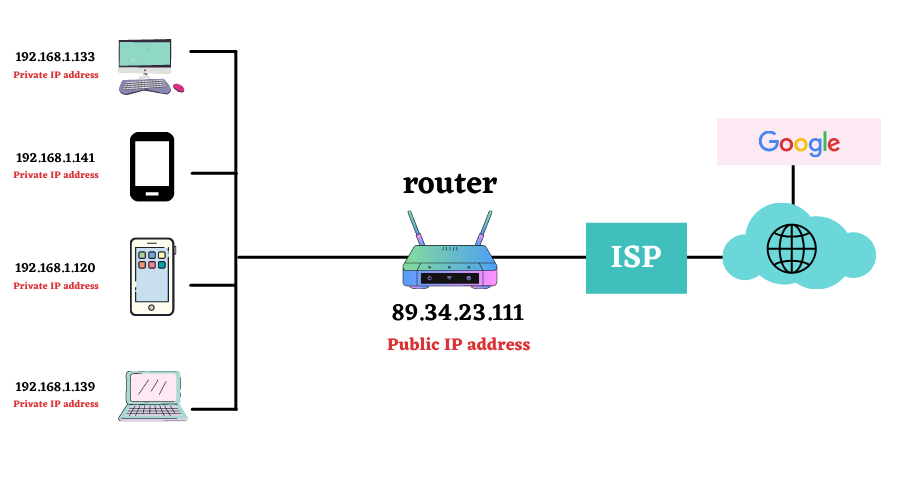
\includegraphics[scale=0.4]{content/chapter14/images/public_private.png}
		\caption{Public \& Private IP}
		\label{fig:public_private_ip}
	\end{figure}
	
	\begin{itemize}
		\item \textbf{Public IP address}: Used \textbf{outside of a network}
		\item \textbf{Private IP address}: Used \textbf{inside a network}
	\end{itemize}
	\bigskip
	\bigskip
	\item \textbf{Permanancy}: There are 2 types of IP address:
	\begin{itemize}
		\item \textbf{Static IP address}: \textbf{Won't change and created manually}. Provided by \textbf{i}nternet \textbf{s}ervice \textbf{p}rovider (ISP) for external usage. 
		\item \textbf{Dynamic IP address}: \textbf{Can change anytime} and assigned by a \textbf{DHCP} server or router.
	\end{itemize}
	\bigskip
	\bigskip
	\item \textbf{IPV4 \& IPV6}
	\paragraph{IPV4}
	\begin{itemize}
		\item IPv4 is used to identify devices on a network using an addressing system.
		\item IPv4 is a 32-bit address.
		\item IPV4 can have approximate 4 million address.
		\item IPV4 carries 94\% of Internet traffic.
	\end{itemize}
	\paragraph{IPV6}
	\begin{itemize}
		\item This new IP address version solves the need for more Internet addresses.
		\item IPv6 is a 128-bit hexadecimal address.
		\item IPV6 allows 340 undecillion unique address space.
	\end{itemize}
\end{itemize}
	
\end{flushleft}


